%%
%%  Example paper
%%
%%

%%%%%%%%%%%%%%%%%% Usenix style %%%%%%%%%%%%%%%%%%%%%%%%%%%%%%%%%
\documentclass[10pt,twocolumn,a4paper]{article}
\usepackage{styles/usenix-style}

\author{Jannik Wibker}

%%%%%%%%%%%%%%%%%% Document %%%%%%%%%%%%%%%%%%%%%%%%%%%%%%%%%%%%%%%%%%%
% TODO: Change draft to final before submitting final version.
\usepackage[draft]{styles/ka-style}
\usepackage{cite,xspace,ifthen,graphicx,listings,caption,multirow}

\captionsetup[figure]{font=small}
\captionsetup[table]{font=small}
\captionsetup[listing]{font=small}

\usepackage[
   pdfauthor={Jannik Wibker},
   pdftitle={Kernel Address Space Layout Randomization: an Overview},
   pdfsubject={KASLR},
   pdfkeywords={Linux, Kernel, ASLR, KASLR, DrK, KPTI}
]{hyperref}

\begin{document}

\title{ Kernel Address Space Layout Randomization: an Overview }

\newcommand{\todo}[1]{{\texttt{[#1]}}}
\newcommand{\code}[1]{{\tt \small{#1}}}

\maketitle
%\draftfooter

\begin{abstract}
KASLR and ASLR are both important measures to strengthen the security of operating systems.
They are however not without flaws and can be circumvented.
In this report I will give an overview of the state of KASLR, its origins and differences in implementation across different operating systems, detail an attack against KASLR called DrK and touch on KPTI (previously KAISER), which is a later introduced mitigation against said attack and multiple others such as Meltdown.
DrK abuses the fact that TSX (Intel Transactional Synchronization Extension) does not notify the kernel of page faults and access violations but rather solely the exception handler of the transaction in user space. Using this DrK can do a timing attack and scan the address space for allocated pages and obtain whether a page is executable or not if mapped.
From this the addresses of the kernel as well as its modules can be inferred.
KPTI mitigates this by reducing the footprint of the kernel in user space and thus reducing the amount of information that can be obtained by DrK, Meltdown and similar attacks.

% add references for: DrK, Meltdown, KAISER, (maybe TSX)

\end{abstract}

\section{Background}\label{sec:background}

The address space of a user space program will typically contain the following:

\begin{itemize}
  \item The executable: \lstinline{.text}, \lstinline{.data}, \lstinline{.bss}, \lstinline{.rodata} and other sections contained or described in the ELF binary.
  \item Dynamically linked libraries, such as libc
  \item Pages allocated by the program itself
  \item The stack. In case of a multi-threaded program each thread has its own stack, all sharing one common address space.
  \item The kernel address space
\end{itemize}

When not using ASLR and KASLR the placement of pages is deterministic and the same each time the program executes assuming no outside factors have changed since and the flow through the application has not differed.
This means that attackers can easily guess where a specific page will be allocated to in the virtual address space of the process, especially when this allocation is a dynamic library or happens shortly after startup.
To combat this, Address Space Layout Randomization was introduced, which randomizes the address where a page is placed at.
ASLR is done at runtime, resulting in the memory layout differing with each execution of the program.
As the kernel is mapped into the address space of every process, it does not change its layout when ASLR is enabled.
Libc and dynamical libraries are a common target used in exploits of which the addresses are most commonly required for the exploit to function. With ASLR this is made harder.

For ASLR to function the executables have to be position independent, meaning that the program works with any base address and does not rely on specific addresses of libraries or pages to function.
These executables are called Position Independent Executables (or PIE for short).
The code of such executable is also referred to as Position Independent Code.

\subsection{Kernel Address Space Layout Randomization}

The kernel is mapped into the address space of every process in order to speed up system calls by reducing the amount of context switches required.
Without the kernel address space being mapped into user space every system call would require a context switch to the kernel address space and back incurring a lot of \textbf{T}ranslation \textbf{L}ookaside \textbf{B}uffer (TLB) flushes.

With Kernel Address Space Layout Randomization the previous shortcoming of ASLR is addressed.
The addresses to where the kernel and its modules or drivers are mapped are randomized at boot time.
With this the addresses of all pages might not differ each time a program is executed but each time the system is rebooted.
As a main focus of many malwares is them being able to spread fast and wide it is paramount that the exploit can be reused across systems without having to be custom tailored to the system itself or even the kernel memory layout which is in use since last booting.
KASLR breaks this assuming it is not possible for the exploit to figure out the kernel memory layout.

\subsection{Entropy}

With both ASLR and KASLR there are certain predefined memory regions where pages can be mapped to.
These regions do differ in size across operating systems and versions thereof, as well as CPU architectures (e.g. x86, x86-64, AAarch64).

Oftentimes the measure of entropy is used to describe the effectiveness of ASLR and KASLR.
Entropy describes the amount of bits of randomness available for a page allocation, i.e. the base 2 logarithm of the size of the region the page can be mapped into.
The size of a region refers to the amount of pages that can possibly be mapped into that region meaning the size in bits divided by the page size in bits.

Higher entropy means that there are more possible addresses for a page to be mapped to.

There can be certain rules in place which reduce the entropy for successive allocations,  thus the entropy is often given for the first allocation only where most rules don't apply yet.
Examples of such rules are an inherent ordering of pages inside a region (module B must come after module A), requested alignment to multiples of the page size, or a minimum amount of empty pages in between each allocation.

With each allocation the entropy for future allocations shrinks as the region is filled up and may rules apply.

\subsection{Introduction To Modern OSes}

\begin{table}[!ht]
    \small
    \centering
    \begin{tabular}{llrr}
    \hline
        \textbf{OS} & \textbf{Release} & \textbf{(K)ASLR} & \textbf{Date} \\ \hline
        \multirow{2}{*}{macOS}   & OS X 10.5              &  ASLR & October 2007 \\ 
                                 & OS X 10.8              & KASLR & July 2012    \\ \\
        \multirow{2}{*}{Linux}   & 2.6.12                 &  ASLR & June 2005    \\ 
                                 & 3.14                   & KASLR & March 2014   \\ \\
        \multirow{2}{*}{Windows} & \multirow{2}{*}{Vista} &  ASLR & \multirow{2}{*}{January 2007} \\
                                 &                        & KASLR & \\ \hline
    \end{tabular}
    \caption{ASLR and KASLR introduction dates into major operating systems}
\end{table}

Windows, Linux and macOS all introduced ASLR and KASLR in the timeframe from 2005 until 2014.
Linux (Kernel 2.6.12) and macOS (Mac OS X Leopard 10.5) both added support for ASLR in 2005.
In 2007 Windows Vista added support for both ASLR and KASLR at the same time. The early implementation of ASLR in Windows Vista was however not the most refined, as the effectiveness on 32-bit systems could be reduced when the system was low on memory.
MacOS implemented KASLR in 2012 with OS X Mountain Lion 10.8.

\subsection{Implementation differences}

When it comes to the implementations of ASLR and KASLR there are some stark differences between the three major desktop operating systems (Windows, Linux and macOS).

\begin{table*}[!ht]
  \small
  \centering
  \begin{tabular}{llcrrr}
  \hline
    \textbf{OS} & \textbf{Type} & \textbf{Address Range} & \textbf{Page Size} & \textbf{Slots} & \textbf{Entropy} \\ \hline
    \multirow{2}{*}{Linux}   & Kernel  & {\lstinline[basicstyle=\ttfamily]![0xffffffff80000000, 0xffffffffc0000000]!} & 16MB &   64 &  6 bits \\
                             & Modules & {\lstinline[basicstyle=\ttfamily]![0xffffffffc0000000, 0xffffffffc0400000]!} &  4KB & 1024 & 10 bits \\ \\
    \multirow{2}{*}{Windows} & Kernel  & {\lstinline[basicstyle=\ttfamily]![0xfffff80000000000, 0xfffff80400000000]!} &  2MB & 8192 & 13 bits \\
                             & Modules & {\lstinline[basicstyle=\ttfamily]![0xfffff80000000000, 0xfffff80400000000]!} &  2MB & 8192 & 13 bits \\ \\
    macOS   & Kernel  & {\lstinline[basicstyle=\ttfamily]![0xffffff8000000000, 0xffffff8020000000]!} &  2MB &  256 &  8 bits \\ \hline
  \end{tabular}
  \caption{Differences in allocation categorized by operating system}
\end{table*}

\textbf{TODO: more details on the differences, similar to what is mentioned later in the report as well (Determining kernel and module mappings)}


\section{The attack - DrK}\label{sec:drk}

The DrK is an attack against KASLR which derandomizes the kernel address space.
It has been proposed in the paper \textit{Breaking Kernel Address Space Layout Randomization with Intel TSX} by \textit{Jang, Yeongjin and Lee, Sangho and Kim, Taesoo} \cite{drk}.
Most of the code necessary to perform the attack can be found on \href{https://github.com/sslab-gatech/DrK}{GitHub} \cite{drk-attack-proof-of-concept-github}.

The attack builds upon Intel TSX and performs a timing attack to infer the state of a page (mapped vs. unmapped and executable vs. non-executable).
This works because with TSX the kernel does not get notified of Page Faults and Access Violations, but the abort handler itself is.
Furthermore the time it takes the \textit{MMU} (Memory Managment Unit) to throw a Page Fault exception slightly differs from the time it takes to throw an Access Violation exception.
Using this the status of a page can be inferred.

\subsection{Intel TSX}

Intel TSX stands for the Intel Transaction Synchronization Extension(s) \cite{intel-tsx-overview}.
It is an interface using which code can be run transactionally, i.e. segmented into clearly defined transactions, aborted and rolled back including all memory writes if so desired.

Aborting and rolling back happens either manually using a directive to abort the transaction or automatically in the case of an exception such as a Page Fault.

\lstset{language=C, basicstyle=\small\ttfamily,
        string=[b]', showspaces=false, showtabs=false,
        caption={Example code for Intel TSX}, captionpos=b}
\begin{lstlisting}
// start transaction, if rolled back
// execution continues from here
// but with a different return value
// (status code of transaction)
if (_xbegin() == _XBEGIN_STARTED) {

  ... // do work

  // commit transaction
  _xend();

  // or abort with status code
  // (=> rollback)
  _xabort(status)
} else {
  // abort handler
}
\end{lstlisting}

The exception being directly handled by an abort handler in userspace is far from the norm. Otherwise this will always notify the kernel which can then decide to terminate the process or take some other kind of action.
With TSX this is not possible as the kernel does not ever get notified of this exception occuring.
This can pose great potential for abuse if used in a nefarious manner as this behavior differs from the status quo and assumptions used elsewhere might not hold with this.
Mechanisms which otherwise rely on the kernel getting notified about page faults such as Demand Paging will not work correctly.

\subsection{Timing differences}

The abort handler does not get information about what exception occured.
Page Faults point to the page being unmapped, while Access Violations point to the page being mapped but inaccessible from userspace.
Differentiating a Page Fault from an Access Violation will have to be done in some other way.
The time the MMU needs to generate a Page Fault for a given memory access differs from the time it takes to generate an Access Violation as the prior one can be deduced faster.
This difference can be measured and used to tell both apart.

Checking for the execution status of the page works similarly.
For a page that is known to be mapped (but inaccessible from userspace, meaning it belongs to the kernel address space) trying to jump to an address contained in the page will take a different amount of time until the exception is generated based on whether the page is executable or not.

\subsection{Crafting the attack}

Combining the previous leads to the following exploit implementation.

By reading from a memory address a Page Fault will be generated if the page is unmapped and an Access Violation if the page is mapped but inaccessible from userspace.
To achieve this, inline assembly is used to move the value at the given address into a register, i.e. a very simple method to read from a concrete memory address.

This function will be called for each page and the timing results interpreted afterwards.

\lstset{language=C, basicstyle=\small\ttfamily,
        string=[b]', showspaces=false, showtabs=false,
        caption={Mapped vs Unmapped timing test}, captionpos=b}
\begin{lstlisting}
uint64_t do_probe_mapped(void* addr) {
  // start timer
  uint64_t beg = rdtsc_beg();

  if (_xbegin() == _XBEGIN_STARTED) {

    // generates access violation
    // mapped vs unmapped
    asm volatile("mov rax, [addr]");
  } else {
    // compute time difference
    return rdtsc_end() - beg;
  }
}
\end{lstlisting}

Similarly the code can be adapted slightly to check for the execution status of a page.
Here instead of reading from an address we try to jump to it.

\lstset{language=C, basicstyle=\small\ttfamily,
        string=[b]', showspaces=false, showtabs=false,
        caption={Executable vs Non-Executable timing test}, captionpos=b}
\begin{lstlisting}
uint64_t do_probe_executable(void* addr) {
  // start timer
  uint64_t beg = rdtsc_beg();

  if (_xbegin() == _XBEGIN_STARTED) {

    // generates access violation
    // executable vs non-executable
    asm volatile(
      "mov rax, addr; jmp rax"
    );
  } else {
    // compute time difference
    return rdtsc_end() - beg;
  }
}
\end{lstlisting}

\subsection{Interpreting the results}

Using \lstinline{do_probe_mapped} and \lstinline{do_probe_executable} the status of a page can be inferred.
To do so the functions are called multiple times and the minimum time is recorded.

\lstset{language=C, basicstyle=\small\ttfamily,
        string=[b]', showspaces=false, showtabs=false,
        caption={Collect timing results}, captionpos=b}
\begin{lstlisting}
uint64_t probe_memory(
  int ntimes,
  int (*do_probe_memory)(void*),
  void* addr
) {
  uint64_t min = UINT64_MAX;
  while (ntimes --) {
    uint64_t clk = do_probe_memory(addr);
    // Only record the minimum
    // timing observed.
    if (clk < min)
      min = clk;
  }
  return min;
}
\end{lstlisting}

Testing with known mapped pages, executable pages as well as unmapped and non-executable pages leads to the following results being shown in \autoref{fig:timing_m_u} and \autoref{fig:timing_x_nx}.

\begin{figure}[h]
  \begin{center}
    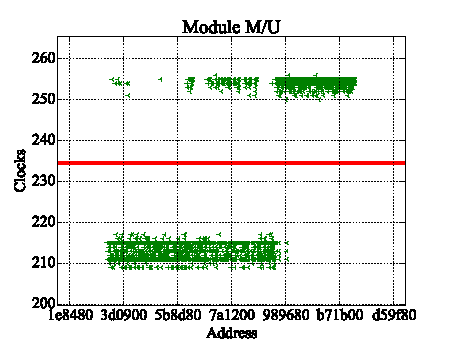
\includegraphics[page=1,width=.4\textwidth]{fig/prebuilt_results_M_U}
  \end{center}
  \caption{Mapped vs Unmapped \cite[Figure~6]{drk}}
  \label{fig:timing_m_u}
\end{figure}

\begin{figure}[h]
  \begin{center}
    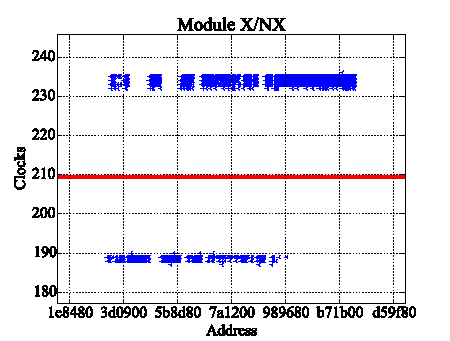
\includegraphics[page=1,width=.4\textwidth]{fig/prebuilt_results_X_NX}
  \end{center}
  \caption{Executable vs Non-Executable \cite[Figure~6]{drk}}
  \label{fig:timing_x_nx}
\end{figure}

Very clear-cut groupings can be observed, using those a categorization into (M)apped vs (U)nmapped and Executable (X) and Non-Executable (NX) can be done.
These values are dependent on the CPU being used. Different hardware will have different timing thresholds.

\begin{figure}[h]
  \begin{center}
    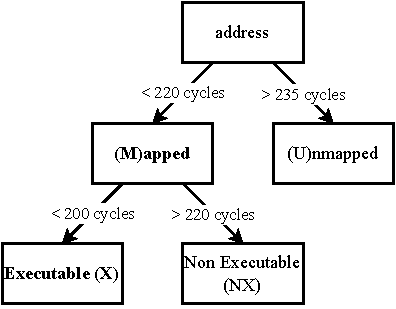
\includegraphics[page=1,width=.4\textwidth]{fig/prebuilt_decision_tree}
  \end{center}
  \caption{Decision tree for categorization of pages}
  \label{fig:decision_tree}
\end{figure}

All read accesses which take less than 220 cycles are considered to be mapped.
Accesses which take more than 235 cycles are considered to be unmapped.
For all pages considered to be mapped an additional check for their execution status is performed.
If jumping to the address takes less than 200 cycles the page is considered executable.
More than 220 cycles is considered non-executable.

\subsection{Determining kernel and module mappings}

With the previous steps the status of a page can be inferred.
This however does not tell anything about what this page is actually being used for.
In many cases extra information such as the precise kernel location or the location of a specific module is required.
Thus a further step is necessary.

The general approach is to associate each known module as well as the kernel itself with a signature and then search the pool of pages for these signatures.
It is to be noted that a module or the kernel itself consists not only of a single page but multiple.

For this operating system specific rules and ranges for page allocation can be used to guess which page corresponds to which module or kernel region.

\subsubsection{Linux}

The address ranges into which the kernel and the modules are mapped are different and do not overlap.
It is therefore easy to tell kernel and module pages apart.
The kernel is located in the range \lstinline{[0xffffffff80000000, 0xffffffffc0000000)}.
Modules are mapped in the range \lstinline{[0xffffffffc0000000, 0xffffffffc0400000]}, thus directly following the address range of the kernel.

Similar to the kernel each module is also mapped as a continoues range of pages, but there is a gap comprised of empty pages in between each module's pages.
Knowing the amount of modules (exposed by \lstinline{lsmod}) and their sizes makes it possible to uniquely identify some of the modules \cite{drk}.

\subsubsection{Windows}
Unlike Linux Windows does not seperate the kernel and the modules into different address ranges.
Both are mapped into the range \lstinline{[0xfffff80000000000, 0xfffff80400000000]}.

Windows sets execute permissions on kernel pages, has at most 6 kernel pages, each with a size of 2MB.
Either the kernel comes before all drivers or after all drivers.

Scanning for the kernel is done by looking for 6 consecutive pages with execute permissions.
After that the location of the modules is either in front or behind the kernel.\cite{drk}

Windows does however have one more trick up its sleeves: The starting position of the kernel is randomized within the page itself.
Figuring out the page is not enough to correctly determine the location of functions or specific instructions.\cite{blog-windows-10-kaslr}

\subsubsection{macOS}

The kernel is mapped in the range \lstinline{[0xffffff8000000000, 0xffffff8020000000]}.
It can be found by looking for the first mapped page.


\section{The mitigation - KPTI}\label{sec:kpti}

A mitigation against many KASLR derandomization attacks is called \textit{Kernel Page Table Isolation} (\textit{KPTI}).
The concept was initially introduced under the name KAISER (\textit{Kernel Address Isolation to have Side-channels Efficiently Removed}) by D. Gruss et al. in \cite{kaiser}.
Originally \textit{KAISER} was implemented as a patch for the Linux kernel and demoed on Ubuntu 16.10.
It was later adapted by the Linux kernel developers and merged into the mainline kernel (4.15) under the name KPTI.

\subsection{The Problem}

The main cause for many KASLR derandomization attacks is improper information leakage after an illegal operation was performed or attempted to be performed by the CPU and not properly rolled back (i.e. caches not being cleared correctly, or timing differences in exception handling, page table traversals and memory accesses).
What all of these attacks rely on is that this initial information is accessed by the CPU and not properly guarded.
If this initial code path leading to the access could be avoided almost all attacks would be rendered unfunctional. \cite{kaiser}

In this case that would mean not mapping the kernel address space into userspace at all and vice-versa, which has been proposed by multiple papers before (Gruss et al. \cite{prefetch-side-channel-smap} and Jang et al. \cite{drk}).

This is a very drastic and brute-force measure which would impact many things such as multithreaded applications or even contexts switches in general making some use cases practically impossible.
Multithreaded applications share the same address space per thread and thus switching to the kernel-only address space would break parallel execution of threads as the user address space would not be accessible anymore.
This would also incur a lot of TLB flushes as the address space would have to be completely switched with every syscall.\cite{kaiser}

Thus a less intrusive approach is needed.

\subsection{The Challenges to overcome}

\textit{D. Gruss et al.} \cite{kaiser} identifies three major challenges that have to be overcome or accomodated for in order for a solution to be viable.

\begin{itemize}
  \item{
    \textbf{Multithreading}:
    Threads share the same address space.
    Thus when a thread enters kernel mode and switches to a kernel-exclusive address space all other threads would switch to the same address space as well, partially defeating the original goal of the mitigation.
    A context switch would also mean having to synchronize all threads.
  }
  \item{
    \textbf{Implicitely assumed and required mappings}:
    Assumptions about the presence of user space mappings being present when in kernel mode and vice-versa are made in many places in the linux kernel.
    These assumptions are often implicit and not easy to spot.
    The architecture of x86 processors requires that a few mappings are present at all times (i.e. when in user space and when in kernel space).
    Changes would have to be made to the kernel at large to accomodate for this, requiring a significant chunk of work.
  }
  \item{
    \textbf{Amount and impact of TLB flushes}:
    Switching the address space incurs an implicit full TLB flush and modifying the address space causes a partial TLB flush. \cite{the-ginormous-intel-manual-volume-3}
  }
\end{itemize}

\subsection{The Approach}

The solution to the given problem by \textit{KAISER} deals with the above challenges.

Split the address space into two parts. First the \textit{Shadow address space} which contains all allocations done in userspace and what is otherwise typically associated with the user space.
Second the \textit{Kernel address space} which contains the kernel code, kernel data and kernel modules.
The kernel address space also has a complete mapping of the user mode space, which is however protected by \textit{SMAP} and \textit{SMEP}.
A few pages are present in both address spaces which are strictly required for the OS to function properly such as the system call trampoline and interrupt descriptor table (\textit{IDT}).

\textit{SMAP} and \textit{SMEP} stand for \textit{Supervisor Mode Access Prevention} and \textit{Supervisor Mode Execution Prevention} respectively.
The MMU restricts accesses originating from the kernel to user-accessible memory.
This is to prevent the kernel from unintentionally executing (or writing to) user space memory.

Whenever a system call occurs in user mode the address space is switched from the shadow address space to the kernel address space.
As each core has its own \textit{CR3}-register (the entrypoint to the currently active page table).
Thus this behaviour solves the multithreading challenge as no two threads can be executed on the same core at the same time with one being in kernel mode while the other is not, which would lead to the same address space being used by both allowing for microarchitectural flaws to be exploited.

To implement switching between the address spaces with as little overhead as possible there needs to be a way to distinguish between them and get the address of the respective other address space using only the \textit{CR3}-register and very little computation.
This is done by enforcing a strict placement of the PML4 page table, which is the top-most and thus entrypoint to the page table hierarchy, such that a single bit encodes the address space in use.
The 12th bit in the address is chosen for this purpose.
A \lstinline{0} refers to the kernel address space and a \lstinline{1} to the shadow address space.
Simple bit manipulation allows computing the address of the other address space and determining which address space is active.

Memory overhead introduced by this is small: 8KB per thread, 12KB per process and 1 MB globally in the kernel.

\textbf{TODO}


\section{Conclusion}\label{sec:conclusion}

Both KASLR and ASLR provide very valuable security against attacks.
The possibility of derandomization attacks existing does not negate the positive impact ASLR and KASLR pose outright, it just slightly lessens their effect.
As with many other vulneratibilities a chain of them has to exist with each one compromising a different layer or part of the system.
Thus a derandomization attack is only a single piece of the puzzle and on its own has no direct impact, only when paired with other exploits making use of the gained information.
It is thus not the end of the world if a derandomization is found and not immediately fixed or mitigated as there are more things that have to go wrong before an attack is possible.
And even with all of the pieces in place having more things to bypass means more complexity on the attacker side which in turn means greater chance of failure or detection as is the case with other software as well.


\section{Related Work}\label{sec:relwork}

This report is mainly based on \cite{drk} as well as \cite{kaiser} for the section on KAISER.
Additionally works with similar topics are \cite{echoload} and \cite{prefetch-side-channel-smap}.


\bibliographystyle{abbrv}
\bibliography{report}
%\footnotesize
\end{document}
